% Restructured book: solution for problem 2.
\chapter{Solution for Problem 2: Snapshot-Guided Image Generation and Editing}

Chapter 5 presents the image-generation and editing workflow built on the editable layout produced in Chapter 4. Its goal is not only to create an attractive interior image. The render should remain traceable to the selected camera view, room shell, major furniture, openings, and relative object positions. The editable layout therefore remains the structural source of truth, while the generated image is a visual interpretation of that layout.

\section{Image Generation}\label{sec:problem2-image-generation}

The image-generation flow begins after the user selects or edits a layout. The frontend reconstructs the layout in a Three.js-based 3D preview and captures a snapshot. The backend then combines this visual snapshot with layout metadata, visible-object contracts, style presets, lighting presets, and negative constraints before calling the image model.

\begin{figure}[!htbp]
\centering
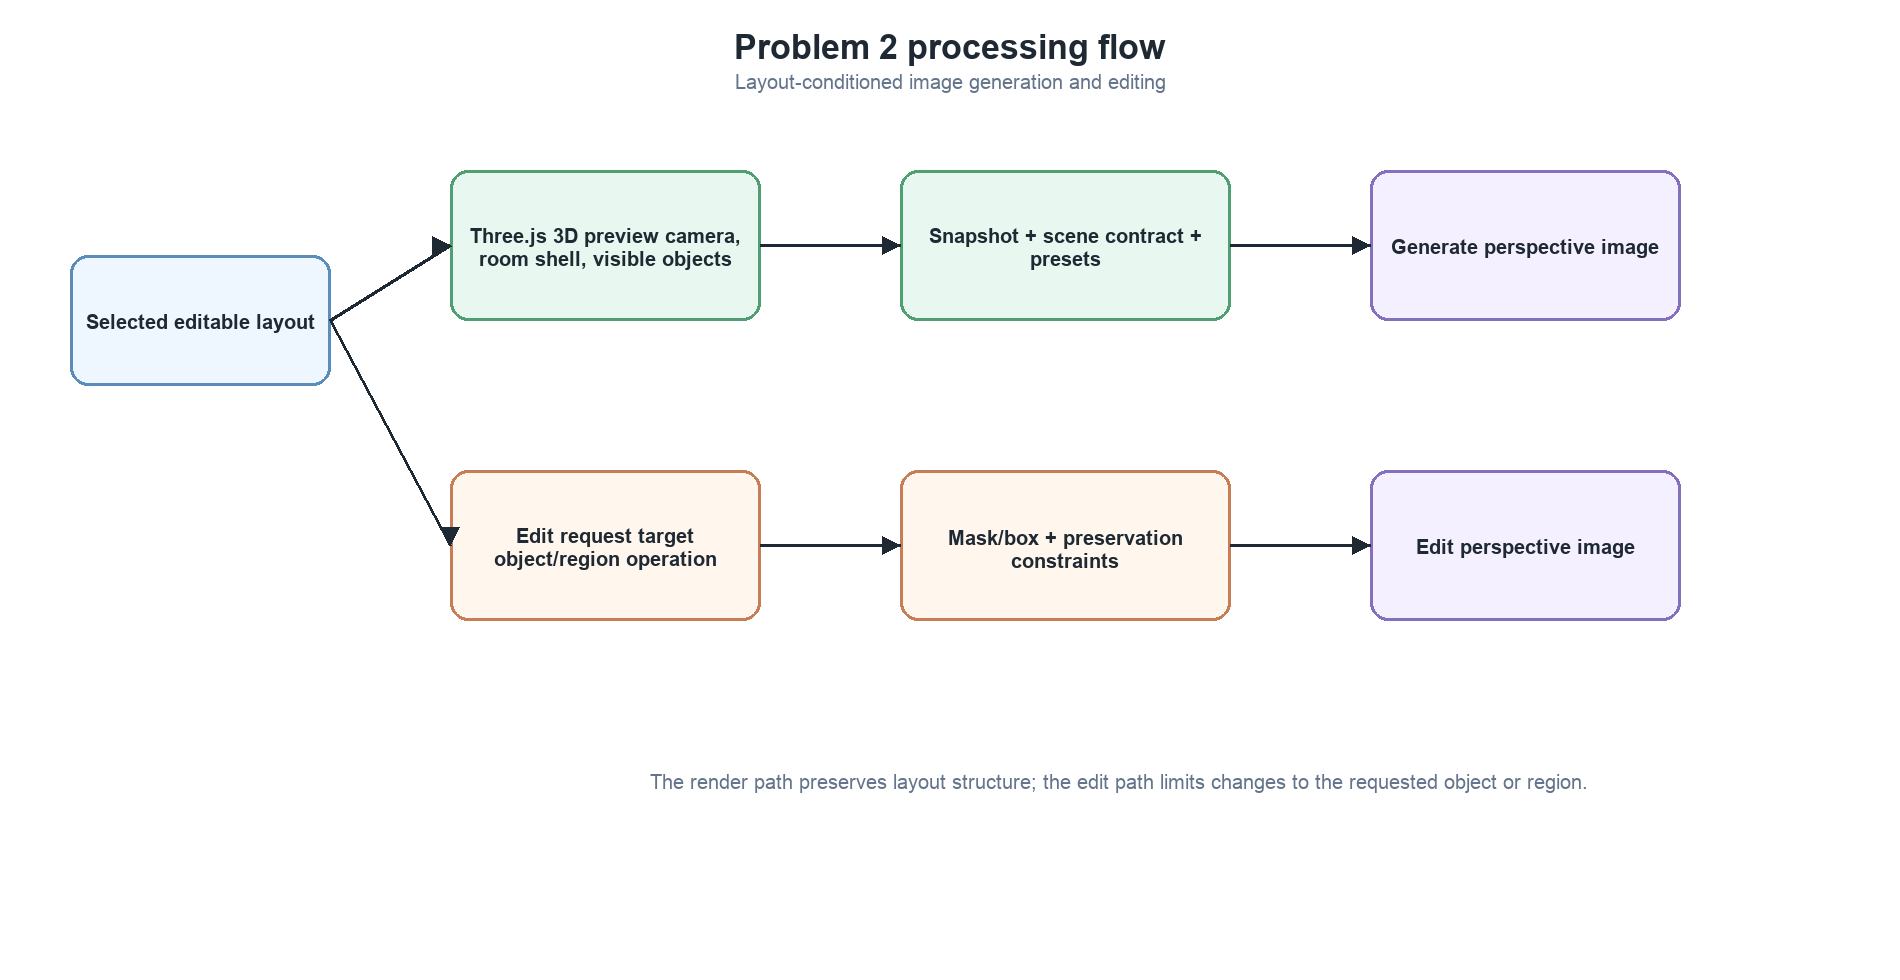
\includegraphics[width=0.96\textwidth]{figures/chapter5/problem2_flow_overview.png}
\caption{Overall processing flow for snapshot-guided image generation and editing.}
\label{fig:5-1}
\end{figure}

The input to image generation is the selected editable layout and the user's visual intent:

\begin{verbatim}
{
  "layout_id": "candidate_07",
  "camera": {"preset": "corner_view", "height_m": 1.6},
  "style_preset": "warm_minimal",
  "lighting_preset": "soft_daylight",
  "scenery_preset": "urban_window_view"
}
\end{verbatim}

The final output is a render artifact linked back to the layout. In the experiments, the main workflow is called single-edit edge/silhouette-guided rendering, abbreviated as SE-ESG in Chapter 7. The abbreviated name is used only in compact tables and charts; the stored artifact keeps the full workflow name for reproducibility.

\begin{verbatim}
{
  "render_id": "render_2026_001",
  "source_layout_id": "candidate_07",
  "workflow_variant": "edge_silhouette_guided_render",
  "image_path": "renders/render_2026_001.png",
  "preservation_targets": ["room_shell", "openings", "major_furniture"],
  "metadata": {"runtime_s": 60.8, "input_tokens": 4078}
}
\end{verbatim}

This structure treats the generated image as a visualization layer derived from the layout. The layout remains the editable design state; the image helps the user understand appearance, lighting, material, and atmosphere.

\hyperref[fig:5-2]{Figure~5.2} expands only the image-generation branch of \hyperref[fig:5-1]{Figure~5.1}.

\begin{figure}[!htbp]
\centering
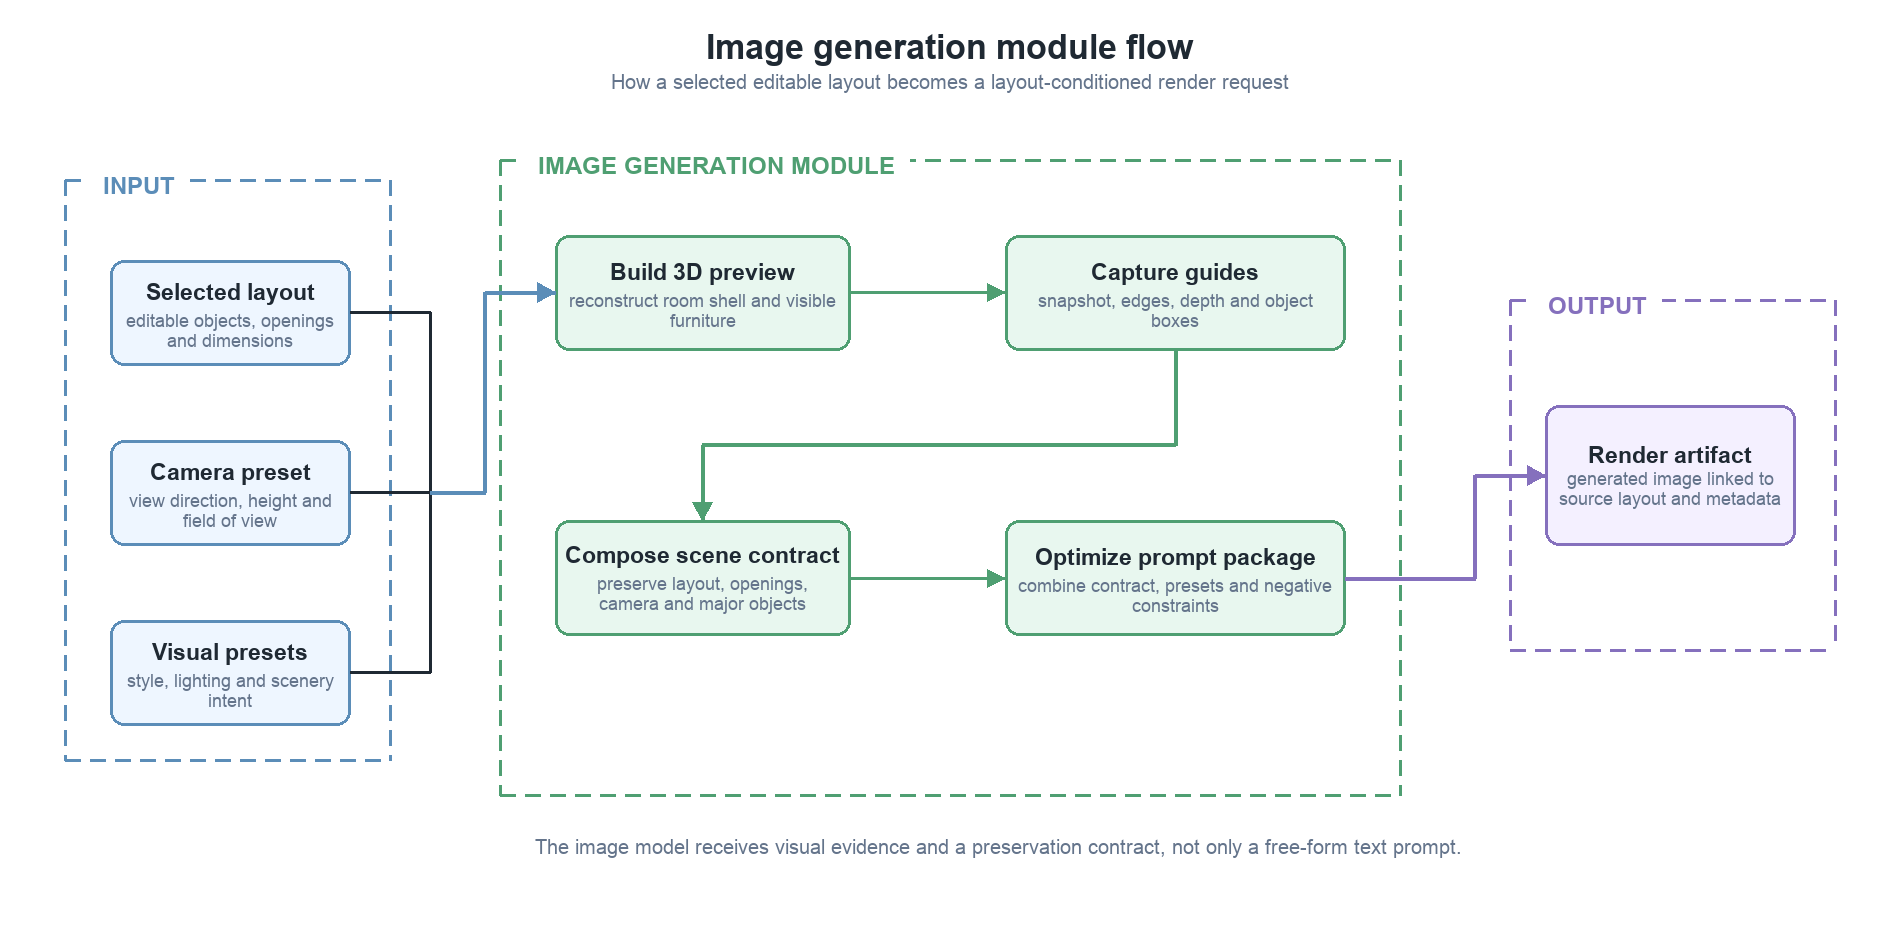
\includegraphics[width=0.98\textwidth]{figures/chapter5/image_generation_flow.png}
\caption{Detailed flow of the image-generation branch.}
\label{fig:5-2}
\end{figure}

\noindent Table~\ref{tab:5-1} lists the main intermediate artifacts that make the image-generation request traceable to the selected layout.

\begingroup
\small
\setlength{\tabcolsep}{4pt}
\renewcommand{\arraystretch}{1.15}
\begin{xltabular}{\textwidth}{|>{\raggedright\arraybackslash}p{2.8cm}|>{\raggedright\arraybackslash}p{2.6cm}|>{\raggedright\arraybackslash}X|>{\raggedright\arraybackslash}X|}
\caption{Main artifacts used by the image-generation workflow.}\label{tab:5-1}\\
\hline
Artifact & Generated by & Main contents & Purpose \\
\hline
3D snapshot & Frontend preview & Source image, camera metadata, visible objects, openings, room shell facts & Provides visual evidence of the selected layout. \\
\hline
Layout guide & Preview and backend compiler & Edge/silhouette, object boxes, optional locked-geometry references & Makes geometry and object boundaries more explicit. \\
\hline
Scene contract & Backend prompt compiler & Camera, room shell, openings, object count, preserve/change rules & Reduces ambiguity in the provider request. \\
\hline
Visible-object contract & Backend prompt compiler & Object ids, categories, screen-space boxes, approximate relations & Helps preserve major furniture identity and position. \\
\hline
Prompt package & Backend renderer & Snapshot references, contracts, presets, negative constraints & Final provider-facing request. \\
\hline
\end{xltabular}
\endgroup

\subsection{Technique 1: Snapshot-Based Layout Conditioning}\label{subsec:problem2-technique-snapshot}

Snapshot-based layout conditioning is the main bridge between the editable layout and the image model. A snapshot is a structured capture of the 3D preview. It contains the source view, camera metadata, visible objects, approximate screen-space boxes, room shell, openings, and optional guide images. This gives the image model visual evidence of what should remain stable.

\begin{verbatim}
{
  "snapshot": {
    "image": "snapshot.png",
    "camera": {"fov": 55, "position": [3.2, 1.6, 4.1]},
    "visible_objects": [
      {"id": "sofa_1", "type": "sofa", "bbox": [0.18,0.42,0.45,0.71]},
      {"id": "tv_1", "type": "tv_console", "bbox": [0.68,0.39,0.90,0.62]}
    ],
    "openings": [{"id": "window_1", "bbox": [0.42,0.15,0.62,0.28]}]
  }
}
\end{verbatim}

This technique is motivated by conditional image-generation research, where spatial evidence such as edges, depth, or segmentation improves output control \cite{Zhang2023AddingConditionalControl}. RoomFlow applies the same principle at the workflow level. The provider receives the selected 3D view, edge or silhouette guides, visible-object metadata, and preservation instructions rather than a text prompt alone. The thesis does not claim that the provider model is retrained or that a ControlNet-style conditioning branch is exposed. The implemented contribution is a snapshot-guided provider workflow built around the editable layout.

Snapshot guidance does not guarantee pixel-level geometric preservation. It supplies additional evidence about the selected camera, room shell, openings, and visible objects, with the expectation of reducing unnecessary changes relative to weaker prompting workflows. Remaining layout drift is measured explicitly in Chapter 7.

\subsection{Technique 2: Scene Contract and Visible-Object Contract}\label{subsec:problem2-technique-contract}

The second technique is contract-based prompting. A scene contract is a concise text-and-JSON description of what the model must preserve: camera framing, room shell, opening count and position, main visible objects, approximate relative positions, and scale relationships. A visible-object contract lists layout-critical objects so that the image request is more concrete than a generic style prompt.

\begin{verbatim}
{
  "scene_contract": {
    "preserve": [
      "same camera view",
      "one north window",
      "sofa facing TV console",
      "rug centered in seating area"
    ],
    "may_change": ["materials", "lighting", "decorative texture"],
    "must_not_change": [
      "room shape",
      "door position",
      "major furniture count"
    ]
  }
}
\end{verbatim}

This contract does not make the image model an exact geometric renderer. It reduces ambiguity. The model can still improve realism, materials, lighting, and atmosphere, but it is repeatedly instructed that the spatial arrangement comes from the selected layout.

The practical effect can be explained by comparing two request forms. Without a scene contract, the prompt may only ask the model to make the room ``warm minimalist'', which leaves object count, opening placement, and camera framing underspecified. With the scene and visible-object contracts, the request explicitly states which objects, openings, and spatial relations must remain stable and which visual properties may change. The expected improvement is therefore not exact geometric rendering, but fewer unnecessary changes to object count, room shell, and camera view. Chapter 7 evaluates this effect through the image-flow variants.

\subsection{Technique 3: Structured Prompt Packaging and Preset Control}\label{subsec:problem2-prompt-optimization}

In this system, prompt optimization means structured prompt packaging rather than automatic search over prompt variants. Each provider-facing request is organized into stable sections: source layout summary, preservation requirements, visible object list, style preset, lighting preset, scenery preset, and negative constraints. This structure makes requests easier to inspect, compare, and reproduce across experiments.

\begin{verbatim}
{
  "prompt_package": {
    "layout_summary": "living room, corner camera, sofa faces TV",
    "style": "warm minimal, light wood, neutral fabric",
    "lighting": "soft daylight from the north window",
    "scenery": "subtle urban exterior",
    "negative_constraints": [
      "do not move the sofa",
      "do not add extra windows",
      "do not change camera angle"
    ]
  }
}
\end{verbatim}

The style, lighting, and scenery presets are separated from geometry. A style preset may request modern, minimalist, boho, or warm material choices. A lighting preset may request daylight, soft evening light, or studio-like clarity. A scenery preset may describe the outside view or environmental mood. These presets should improve visual appearance without changing the underlying layout goal.

Figure~\ref{fig:5-3} shows a real create-flow example with the source snapshot, edge/silhouette guidance, and generated render placed side by side.

\begin{figure}[!htbp]
\centering
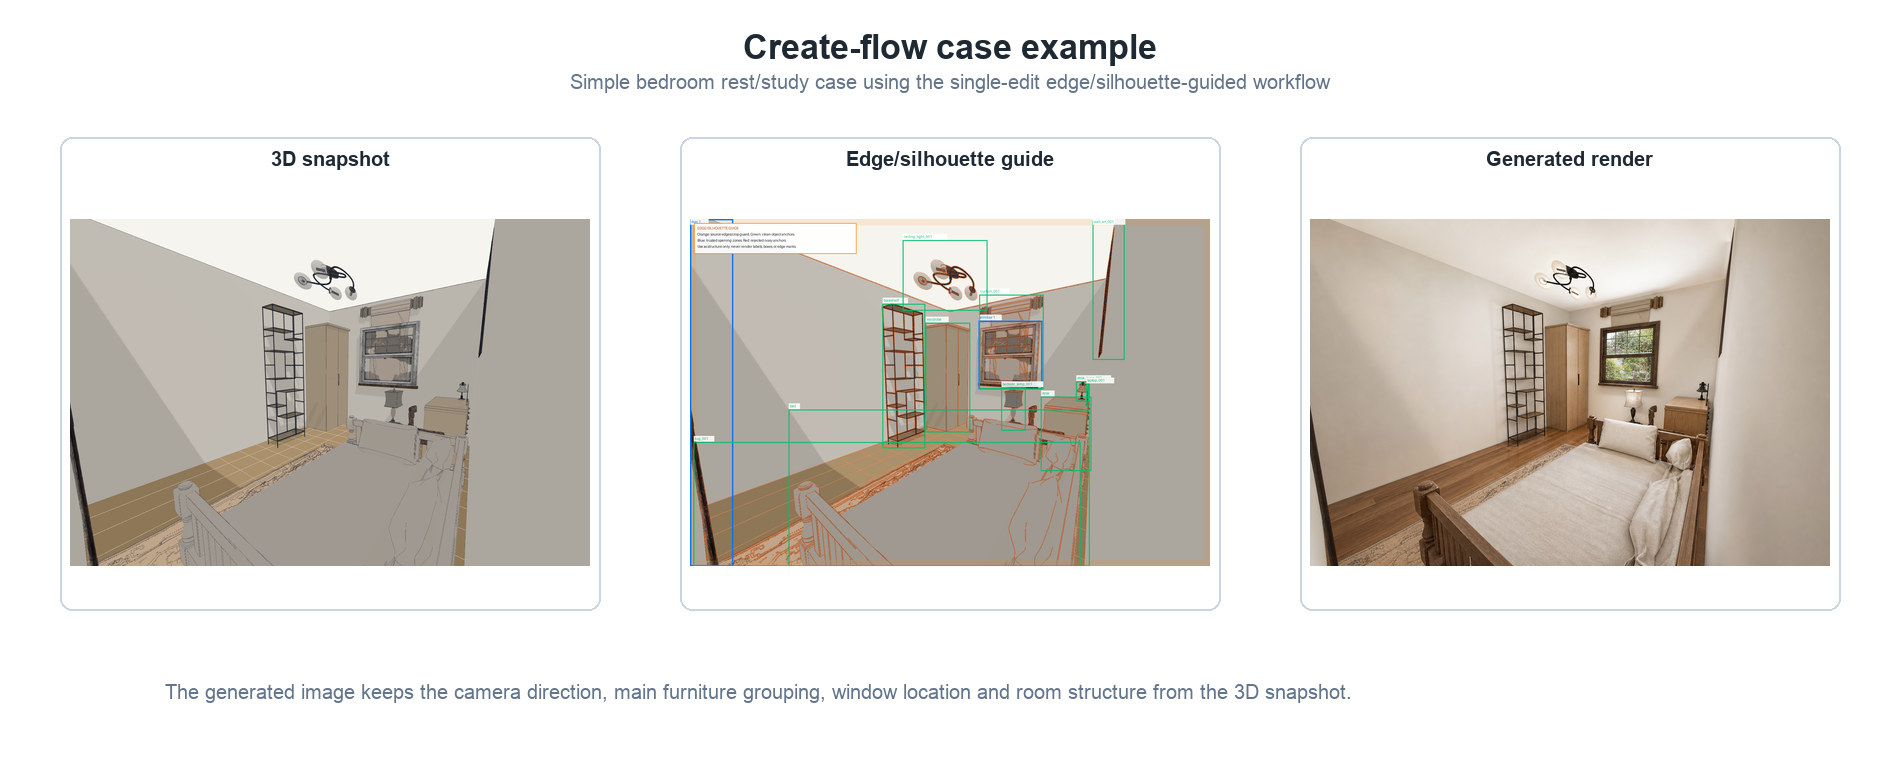
\includegraphics[width=0.96\textwidth]{figures/chapter5/create_case_example.png}
\caption{Real create-flow example from a bedroom rest/study case.}
\label{fig:5-3}
\end{figure}

In Figure~\ref{fig:5-3}, the left panel is the 3D snapshot, the middle panel is the edge/silhouette guide, and the right panel is the generated render. The window direction, camera view, room shell, and main furniture grouping are the preservation targets.

\section{Image Editing}\label{sec:problem2-image-editing}

Image editing starts from an approved render rather than from a blank prompt. The user chooses an edit operation, such as add, remove, replace, or recolor. The system prepares the source render, target object or region, requested operation, optional replacement reference, and preservation constraints. The purpose is to make the edit local and controllable.

Figure~\ref{fig:5-4} summarizes the image-editing module from source render and target scope to edited output and saved artifact.

\begin{figure}[!htbp]
\centering
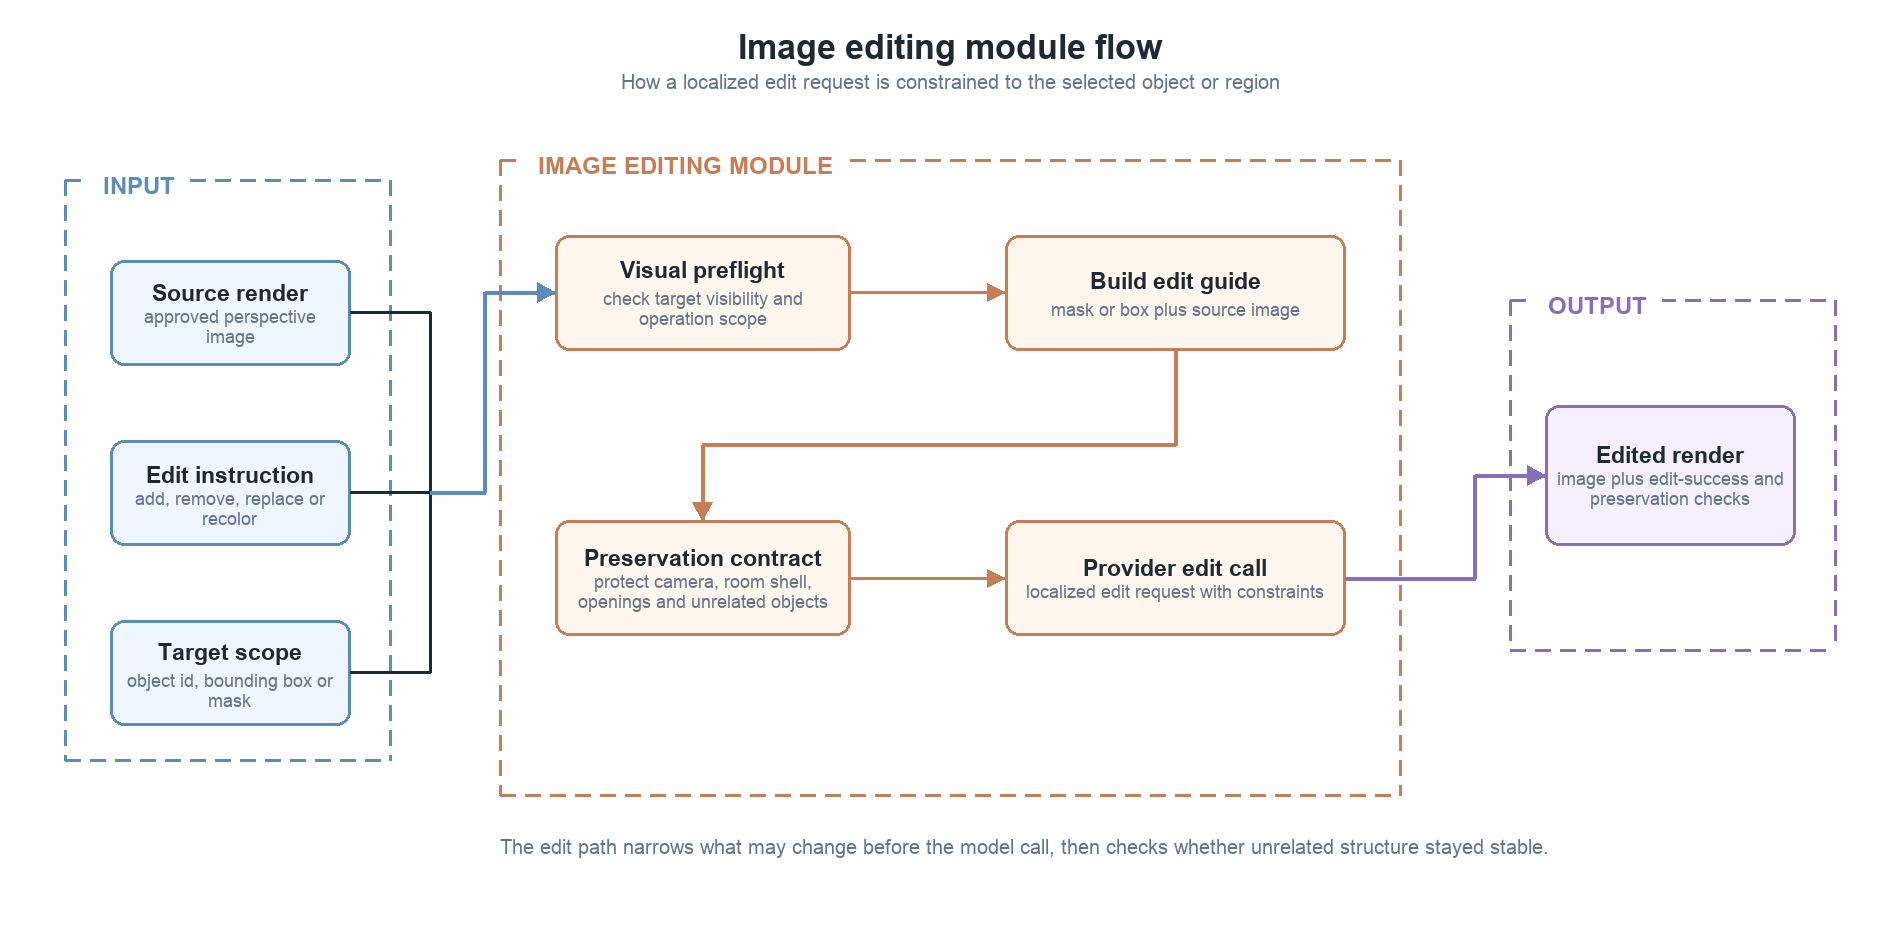
\includegraphics[width=0.98\textwidth]{figures/chapter5/image_editing_flow.png}
\caption{Detailed flow of the image editing module.}
\label{fig:5-4}
\end{figure}

\subsection{Edit Request and Target Scope}\label{subsec:problem2-edit-target-scope}

Each edit request is connected to a target scope whenever possible. If the target corresponds to a known layout object, the system can reuse its object id and approximate visible box. If the target exists only in the generated render or is not linked reliably to layout data, the user can select a manual region on the image. When localization is reliable, the system uses a mask; otherwise, it falls back to a normalized bounding box and a textual target description. This scope reduces ambiguity because the image model is told both what to change and where the change should occur. Instruction-based editing shows that an input image and a written instruction can define an edit \cite{Brooks2023Instructpix2pixLearningFollow}; RoomFlow adds layout-derived object scope so that the edit better fits an interactive interior-design workflow.

\begin{verbatim}
{
  "source_render_id": "render_2026_001",
  "operation": "add",
  "target": {
    "region_id": "manual_add_box_1",
    "bbox": [0.73, 0.26, 0.86, 0.47]
  },
  "instruction": "Add a framed landscape wall art in the target region"
}
\end{verbatim}

\subsection{Visual Preflight and Preservation Constraints}\label{subsec:problem2-edit-preflight}

Before the provider call, the visual preflight stage prepares the edit scope and detects obvious target ambiguity. If a mask can be produced, it marks the region that should change. If a bounding box is used, it provides a weaker but still useful spatial cue. The edit request also states which parts of the room should remain fixed, such as camera view, room shell, openings, and unrelated furniture.

\begin{verbatim}
{
  "edit_preflight": {
    "target_found": true,
    "mask_path": "masks/manual_add_box_1.png",
    "preserve": [
      "camera_view",
      "room_shell",
      "door_and_window_positions",
      "unrelated_furniture"
    ],
    "allowed_change_region": "target_box_or_mask"
  }
}
\end{verbatim}

The visual preflight stage is used for control rather than aesthetics. Its purpose is to reduce unintended changes before the provider call. For example, it helps prevent a recolor request from changing the whole room, a replacement request from moving the camera, or a remove request from deleting unrelated furniture. The stage therefore defines the allowed edit region and the protected elements before image editing begins.

Table~\ref{tab:5-2} defines the compact visual-preflight schema used to pass target localization and preservation constraints into the edit request.

\begingroup
\small
\setlength{\tabcolsep}{4pt}
\renewcommand{\arraystretch}{1.15}
\begin{xltabular}{\textwidth}{|>{\raggedright\arraybackslash}p{3.0cm}|>{\raggedright\arraybackslash}X|}
\caption{Visual preflight output schema for localized image editing.}\label{tab:5-2}\\
\hline
Field & Interpretation \\
\hline
target\_found & Whether the requested object or region can be localized before editing. \\
\hline
target\_source & Layout object id, visible-object box, or manual region used as the target source. \\
\hline
mask\_path / bbox & Strong mask if available; otherwise normalized image box. \\
\hline
operation & Add, remove, replace, or recolor request passed to the provider. \\
\hline
preserve & Camera, room shell, openings, unrelated furniture, and other protected elements. \\
\hline
failure\_reason & Explanation returned when the target is missing or too ambiguous. \\
\hline
\end{xltabular}
\endgroup

Figure~\ref{fig:5-5} illustrates the visual meaning of this schema: the orange target region indicates where the add operation is allowed, while the rest of the room is protected by preservation constraints.

\begin{figure}[!htbp]
\centering
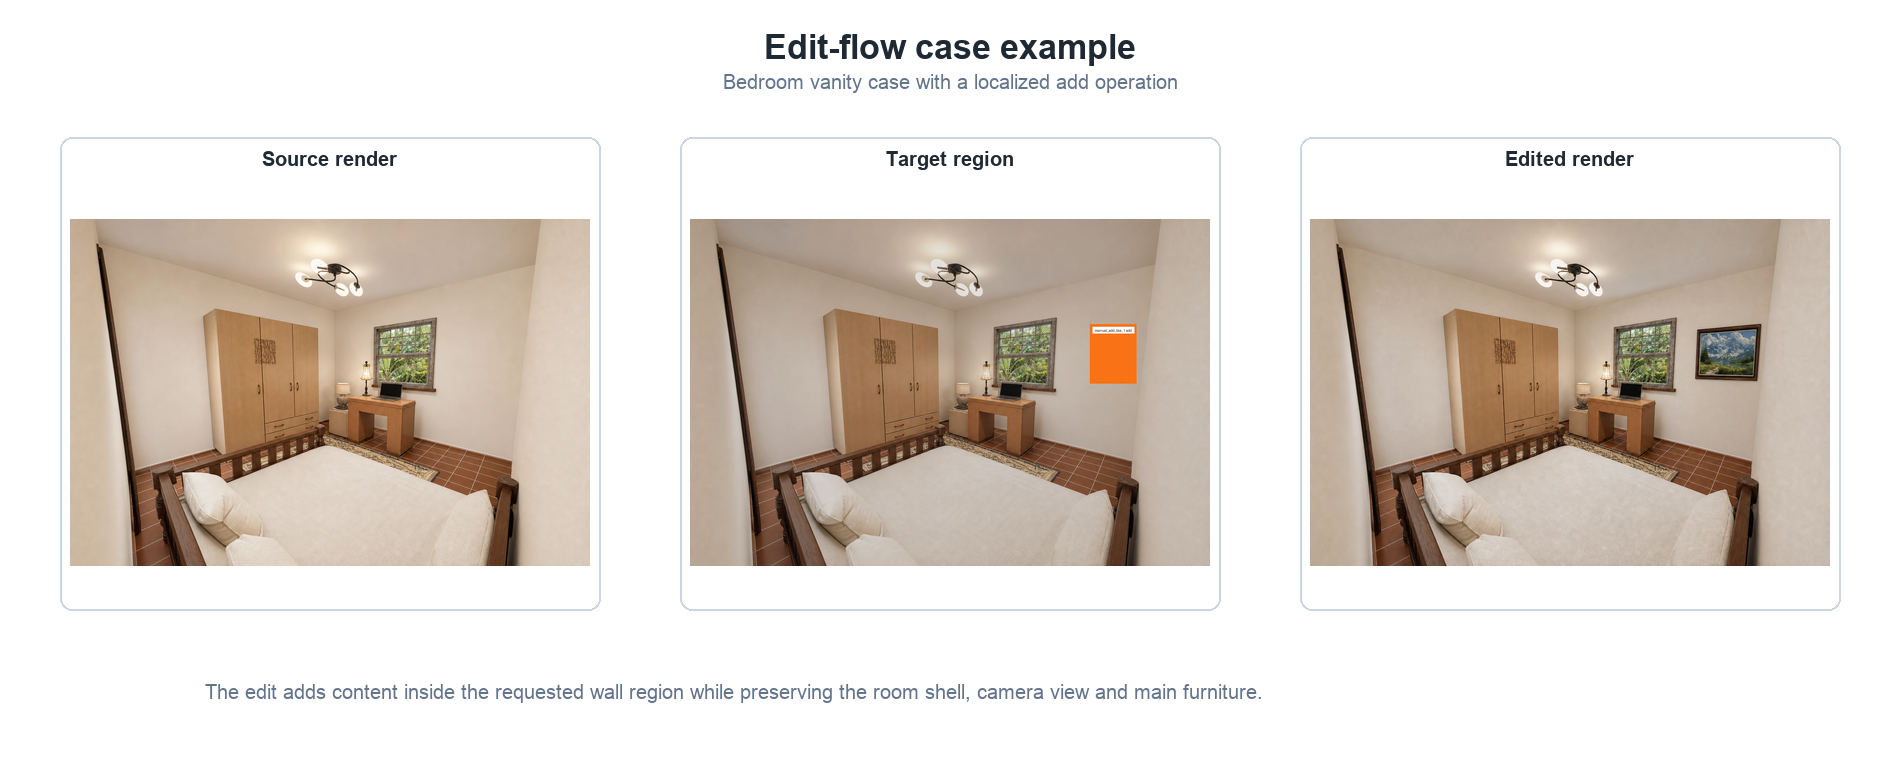
\includegraphics[width=0.96\textwidth]{figures/chapter5/edit_case_example.png}
\caption{Real edit-flow example: the source render is edited by applying the requested operation to the marked target region while preserving the camera, room shell, and unrelated furniture.}
\label{fig:5-5}
\end{figure}

\subsection{Edited Render Output}\label{subsec:problem2-edited-render-output}

The expected result is a localized image edit that preserves the design context. A recolor operation should change the selected object without recoloring the whole room. A remove operation should remove the target object while repairing the surrounding wall or floor. A replacement operation should change the intended furniture item while keeping its approximate location and scale.

The \texttt{checks} field stores evaluation or inspection results associated with the edited render. In the simplified example below, the values illustrate the intended state after the edit has been judged successful. In the benchmark, edit success and structure preservation are measured separately rather than assumed from the provider response.

\begin{verbatim}
{
  "edited_render_id": "edit_2026_001",
  "source_render_id": "render_2026_001",
  "operation": "add",
  "target_region_id": "manual_add_box_1",
  "image_path": "renders/edit_2026_001.png",
  "checks": {
    "edit_applied": true,
    "target_localized": true,
    "structure_preserved": true
  }
}
\end{verbatim}

Figure~\ref{fig:5-6} shows the final edited render artifact for the same localized add operation.

\begin{figure}[!htbp]
\centering
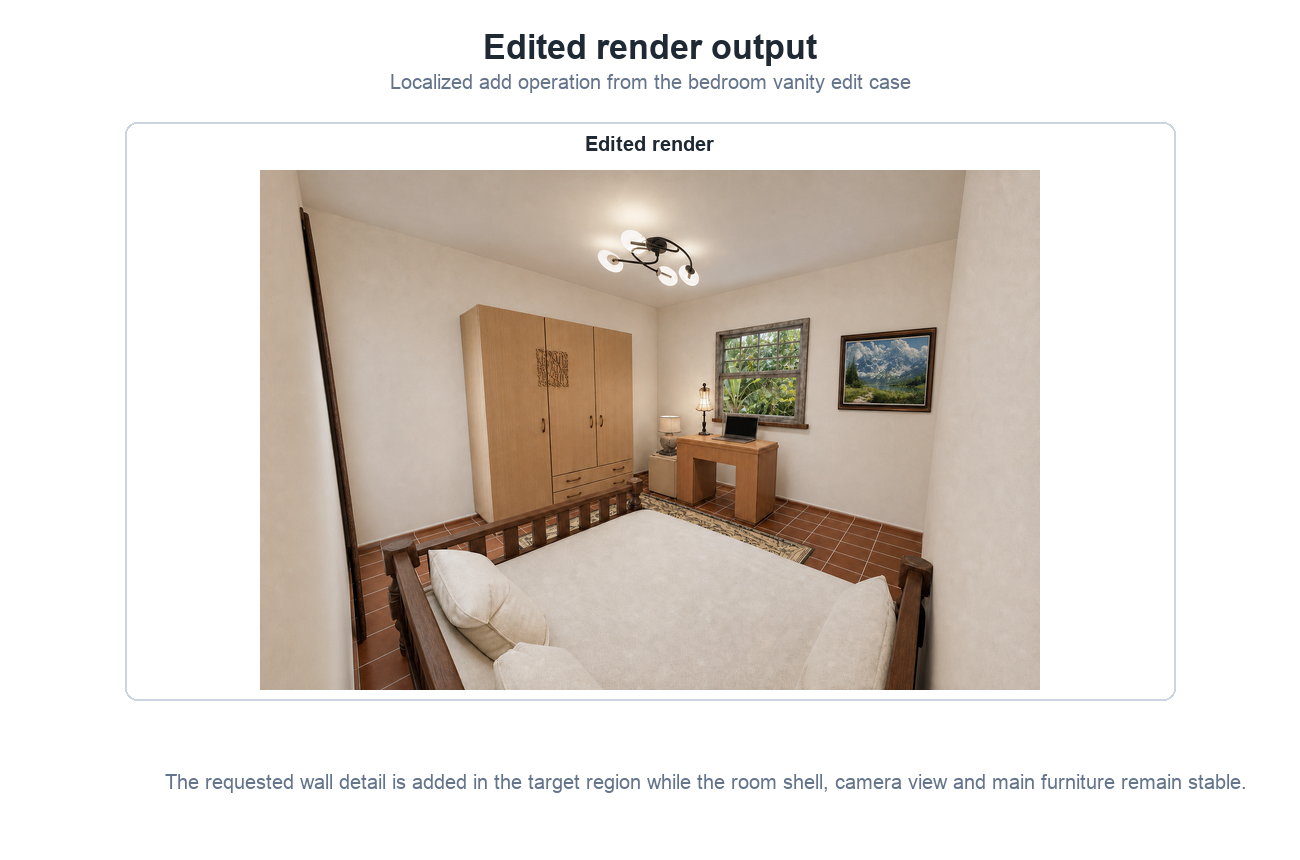
\includegraphics[width=0.96\textwidth]{figures/chapter5/edit_output_example.png}
\caption{Edited render output from a real localized add operation, showing the generated artifact that remains linked to the source render and target region.}
\label{fig:5-6}
\end{figure}

The edit output in Figure~\ref{fig:5-6} remains linked to the source render and the underlying layout. This link is important for later evaluation because the edited image can be checked for edit success, target localization, structure preservation, and unintended changes outside the target scope.

The generated or edited render is a visual artifact, not the structural source of truth. The editable layout remains the authoritative design state. If an image drifts in camera framing, room geometry, object identity, or opening position, the drift is treated as a rendering failure rather than a valid layout update. The current system can save and evaluate such renders, but it does not automatically synchronize image-only edits back into the editable 2D layout.
